\documentclass[xcolor={dvipsnames,rgb}]{beamer}

\beamertemplatenavigationsymbolsempty

\usepackage{tikz}
\usepackage{amsmath}
\usepackage{amssymb}
\usepackage{mathtools}

\usetikzlibrary{positioning}
\usetikzlibrary{backgrounds}
\usetikzlibrary{tikzmark}
\usetikzlibrary{shapes,arrows,calc}

\newcommand{\highlight}[2]{\colorbox{#1}{$\mathstrut #2$}}

\definecolor{variable}{HTML}{999999}
\definecolor{operator}{HTML}{bbbbbb}
\definecolor{vtrue}{HTML}{66ff66}
\definecolor{vfalse}{HTML}{ff6666}
\definecolor{rtrue}{HTML}{aaffaa}
\definecolor{rfalse}{HTML}{ffaaaa}

\tikzstyle{into} = [draw, -triangle 45, shorten >=0pt]

\tikzstyle{label} = [minimum height=2em, minimum width=2em]
\tikzstyle{var} = [draw, rectangle, minimum height=2em, minimum width=2em, fill=variable]
\tikzstyle{oper} = [draw, rectangle, minimum height=2em, minimum width=2em, fill=operator]
\tikzstyle{it} = [draw, diamond, minimum height=2em, minimum width=2em, fill=vtrue]
\tikzstyle{if} = [draw, circle, minimum height=2em, minimum width=2em, fill=vfalse]
\tikzstyle{ot} = [draw, diamond, minimum height=2em, minimum width=2em, fill=rtrue]
\tikzstyle{of} = [draw, circle, minimum height=2em, minimum width=2em, fill=rfalse]



% https://i.stack.imgur.com/2X1Jv.png
\colorlet{ca}{Peach!30}
\colorlet{co}{Goldenrod!30}
\colorlet{cn}{Tan}
\colorlet{ci}{Sepia!30}



\begin{document}

\begin{frame}{\textit{Behavior} for the \textbf{unary} operator \texttt{\bf F} ($\diamond$)}

  \begin{center}
    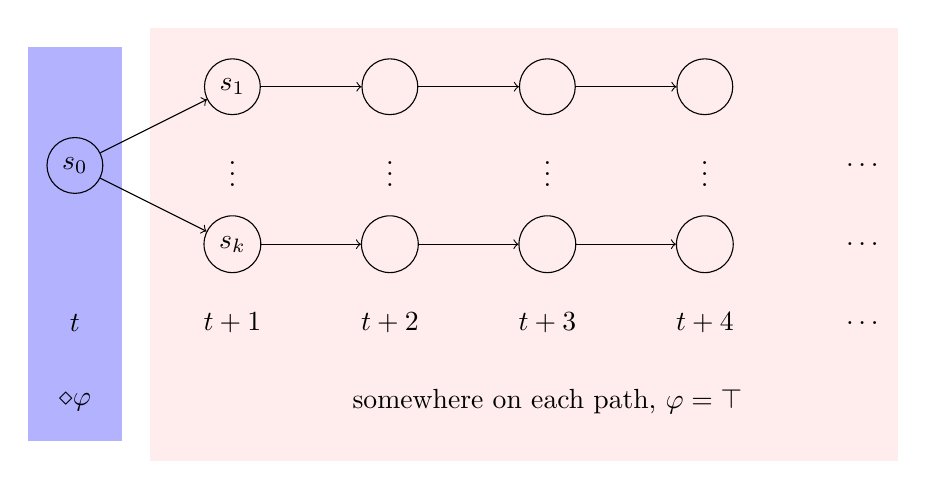
\begin{tikzpicture}

      \onslide<9->{\node [draw=none, fill=blue!30, minimum width=12mm, minimum height=50mm] at (0, 1) {};}

      \onslide<9->{\node at (0, -1) {$\diamond \varphi$};}

      \onslide<10->{\node [draw=none, fill=pink!30, minimum width=95mm, minimum height=55mm] at (5.7, 1) {};}
      
      \onslide<10->{ \node at (6, -1) {somewhere on each path, $\varphi = \top$};}

      \onslide<1-> { \node at (0, 0) {$t$}; }
      \onslide<2-> {\node at (2, 0) {$t+1$}; }
      \onslide<3-> { \node at (4, 0) {$t+2$}; }
      \onslide<4->{ \node at (6, 0) {$t+3$}; }
      \onslide<5->{ \node at (8, 0) {$t+4$}; }
      
      \onslide<6->{ \node[shape=circle,draw=black] (0) at (0, 2) {$s_0$}; }

      \onslide<7->{ \node[shape=circle,draw=black] (k)  at (2, 1) {$s_k$}; }
      \onslide<8->{ \node[shape=circle,draw=black] (k1) at (4, 1) {\phantom{$s_k$}}; }
      \onslide<8->{ \node[shape=circle,draw=black] (k2) at (6, 1) {\phantom{$s_k$}}; }
      \onslide<8->{ \node[shape=circle,draw=black] (k3) at (8, 1) {\phantom{$s_k$}}; }

      \onslide<6->{ \node at (10, 0) {$\ldots$}; }
      \onslide<8->{ \node at (10, 1) {$\ldots$}; }
      \onslide<8->{ \node at (10, 2) {$\ldots$}; }

      \onslide<7->{\node at (2, 2) {$\vdots$};}
      \onslide<8->{\node at (4, 2) {$\vdots$};}
      \onslide<8->{\node at (6, 2) {$\vdots$};}
      \onslide<8->{\node at (8, 2) {$\vdots$};}

      \onslide<7->{ \node[shape=circle,draw=black] (1)  at (2, 3) {$s_1$}; }
      \onslide<8->{ \node[shape=circle,draw=black] (11) at (4, 3) {\phantom{$s_1$}}; }
      \onslide<8->{ \node[shape=circle,draw=black] (12) at (6, 3) {\phantom{$s_1$}}; }
      \onslide<8->{ \node[shape=circle,draw=black] (13) at (8, 3) {\phantom{$s_1$}}; }
      
      \onslide<7->{ \path [->](0) edge node {} (1); }
      \onslide<7->{ \path [->](0) edge node {} (k); }

      \onslide<8->{\path [->](k) edge node {} (k1);}
      \onslide<8->{\path [->](k1) edge node {} (k2);}
      \onslide<8->{\path [->](k2) edge node {} (k3);}
      
      \onslide<8->{\path [->](1) edge node {} (11);}
      \onslide<8->{\path [->](11) edge node {} (12);}
      \onslide<8->{\path [->](12) edge node {} (13);}
      
       
    \end{tikzpicture}

    \only<1-5>{{\bf Time} advances from the {\em current state}
      onward.}

    \only<7-8>{There may be {\bf several} possible future paths.}

    \only<10-12>{$\diamond \varphi$ states that $\varphi$ is true at
      {\bf at least one} future state\footnote{regardless of the path
      taken}.}

    \only<13-15>{This operator is called \textit{future}.}

  \end{center}
\end{frame}


\end{document}
